% Informe basado en la plantilla IEEEtran de ULEAM suministrada por el usuario.
% Compilar: pdflatex main; bibtex main; pdflatex main; pdflatex main.
\documentclass[journal,onecolumn,11pt,a4paper]{IEEEtran}
\usepackage[utf8]{inputenc}
\usepackage[T1]{fontenc}
\usepackage[spanish,es-nodecimaldot,es-tabla]{babel}
\usepackage{newtxtext,newtxmath}
\usepackage{graphicx,booktabs,array,tabularx,amsmath,siunitx,caption,placeins}
\usepackage{microtype}
\usepackage[hidelinks]{hyperref}
\sisetup{output-decimal-marker={,},per-mode=symbol}
\graphicspath{{figuras/}}
\captionsetup{font=small,labelfont=bf,labelsep=period}
\setlength{\emergencystretch}{2em}
\renewcommand{\IEEEkeywordsname}{Palabras clave}
\renewcommand{\abstractname}{Resumen}
% EDITAR ANTES DE ENTREGAR: las fuentes no identifican a los autores del equipo.
% No se atribuye automáticamente este proyecto a los autores del artículo de referencia.
\newcommand{\Autores}{Equipo E-TWIN}
\newcommand{\Afiliacion}{Afiliación institucional y carrera: por completar}
\newcommand{\Correos}{Correos institucionales: por completar}
\newcommand{\Tutor}{Tutor académico: por completar}
% Reemplazar \Autores por los nombres completos de los 2--4 estudiantes.

\hypersetup{pdftitle={E-TWIN: monitoreo energético y vibracional con arquitectura IoT y seguridad operacional},pdfauthor={Equipo E-TWIN}}
\begin{document}
\title{E-TWIN: monitoreo energético y vibracional con arquitectura IoT y seguridad operacional}
\author{\Autores\\[0.4em]
\normalsize\Afiliacion\\
\normalsize\Correos\\
\normalsize\Tutor\\[0.3em]
\normalsize Categoría 3: Industria 4.0, AIoT y Gemelos Digitales}
\markboth{I Concurso Nacional IoT ULEAM 2026 --- Informe técnico}{E-TWIN: monitoreo energético y vibracional}
\maketitle
\begin{abstract}
El monitoreo conjunto de consumo eléctrico y vibración permite contextualizar el comportamiento de una máquina sin intervenir en su control. Este trabajo presenta E-TWIN, un prototipo distribuido con dos nodos sensores y una pasarela M5 Core2. Un ATOMS3 Lite adquiere seis variables de un PZEM-004T; un ATOMS3 procesa aceleración triaxial a 500 Hz mediante filtrado digital de 6--75 Hz. Ambos transmiten por ESP-NOW con cifrado unicast, autenticación de mensajes y controles de secuencia. La pasarela integra una interfaz táctil, una referencia de diez pares válidos y publicación MQTT sobre TLS hacia ThingSpeak, consultada por un SCADA web de solo lectura. La evaluación comprende evidencias del prototipo, pruebas de software y los últimos diez minutos de lecturas conjuntas válidas del archivo suministrado: 31 registros separados por 20 s. Se observaron una potencia media de 341,15 W, aceleración RMS media de 4,736 m/s\textsuperscript{2} y un incremento energético de 57 Wh. La integración de potencia difirió del contador en 0,389\%, resultado de consistencia interna y no de exactitud metrológica. El aporte es una cadena de telemetría trazable que combina calidad de datos, representación operativa y controles de seguridad. La calibración independiente, el diagnóstico de fallas y la validación de campo prolongada constituyen etapas posteriores.
\end{abstract}
\begin{IEEEkeywords}
Internet de las cosas, monitoreo energético, vibración mecánica, procesamiento en el borde, seguridad operacional, gemelo digital.
\end{IEEEkeywords}

\section{Introducción}
La evaluación del comportamiento de una máquina requiere relacionar su demanda eléctrica con su condición de operación. Una lectura aislada de potencia no distingue entre cambios de carga, variaciones del proceso o deterioro mecánico. Del mismo modo, una aceleración elevada no identifica por sí sola una falla. El problema abordado por E-TWIN es integrar ambas perspectivas en una representación accesible, preservando la procedencia, vigencia y calidad de cada medición.

En el contexto del concurso, la propuesta se vincula con la digitalización de pequeñas instalaciones productivas, talleres y sistemas de bombeo, escenarios de aplicación potencial y no despliegues acreditados en esta evaluación. La categoría de Industria 4.0, AIoT y Gemelos Digitales valora explícitamente la integración con SCADA y la seguridad de tecnología operacional (OT)~\cite{bases2026}. Se prioriza una solución replicable que conserve la supervisión local y limite la dependencia de servicios remotos.

Varela-Aldás \textit{et al.}~\cite{varela2022} presentan un monitor eléctrico con M5Stack Core2, sensores PZEM-004T y ThingSpeak, evaluado frente a un equipo de referencia. Este antecedente sustenta la selección de la instrumentación eléctrica, pero no transfiere su exactitud a otras unidades. Tsai \textit{et al.}~\cite{tsai2023} también desarrollan monitoreo inalámbrico de potencia y lo contrastan con instrumentación independiente. E-TWIN añade adquisición inercial distribuida, un contrato explícito de calidad y controles de autenticidad a la integración eléctrica y visual.

La denominación de gemelo digital se utiliza aquí con alcance operativo: una representación alimentada por el activo físico. La distinción entre gemelo y sombra digital~\cite{sepasgozar2021} impide equiparar esta visualización con un modelo físico validado o un lazo de control bidireccional. La versión evaluada es de solo monitoreo: no predice vida útil, no estima torque ni gobierna actuadores. Asimismo, la orientación de NIST hacia la seguridad OT~\cite{nist2023} se emplea como marco de diseño, no como certificación del prototipo.

El objetivo es integrar telemetría eléctrica y vibracional, procesarla localmente y exponerla de forma comprensible y verificable. Las contribuciones son la arquitectura de tres dispositivos, el procesamiento inercial por ventanas con banderas de calidad, la referencia operativa de diez pares, y una evaluación reproducible que separa evidencia funcional, consistencia numérica y validación metrológica pendiente.

\section{Metodología}
\subsection{Enfoque y material de evaluación}
Se realizó un estudio descriptivo del prototipo y una revisión reproducible del firmware \texttt{V2}, las fotografías, cuatro capturas de pantalla y la exportación \texttt{feeds.csv} proporcionados por el equipo~\cite{evidencias}. Las fases fueron: reconstrucción de la arquitectura desde el código; identificación de criterios de validez; selección temporal de datos; cálculo de indicadores; y contraste del alcance de los resultados con la literatura. No se infirieron parámetros de placa, régimen de carga ni condiciones ambientales que no constan en las evidencias.

La evaluación distingue tres niveles. La verificación funcional se apoya en las imágenes, la telemetría y las pruebas ejecutables del software. La consistencia interna contrasta relaciones entre variables provenientes del mismo sistema. La validación metrológica exige observaciones simultáneas de un instrumento independiente; ese conjunto no está presente. Esta separación evita convertir una coincidencia algebraica en una afirmación de precisión.

\subsection{Selección de los últimos diez minutos válidos}
El CSV contiene 1819 registros históricos de estructuras heterogéneas. Se convirtieron las ocho columnas de medición a valores numéricos y las fechas a UTC, conservando intacto el archivo original. Se interpretó el campo \texttt{status}, que incluye versión del protocolo, validez por nodo, antigüedad, alarmas y calidad de adquisición. Los valores ausentes o no numéricos se rechazaron; no se reemplazaron por cero.

Se exigieron ocho valores finitos, protocolo 2, ambos nodos válidos y antigüedad inferior a 5000 ms. Los límites de admisión fueron los del firmware: tensión 0--300 V, corriente 0--110 A, potencia 0--33000 W, energía no negativa, frecuencia 40--70 Hz y factor de potencia 0--1,01. Para vibración se exigieron RMS no negativo, pico no inferior al RMS, ambos inferiores a 150 m/s\textsuperscript{2}, bandera válida sin errores, 500 muestras, cero muestras perdidas y tasa estimada entre 475 y 525 Hz. Estos son controles de plausibilidad del programa, no especificaciones de exactitud ni límites de seguridad de la máquina.

De los 62 registros que satisfacen conjuntamente esos criterios en todo el archivo, el último corresponde al 23 de octubre de 2026 a las 21:50:37 UTC. Se definió la ventana cerrada
\begin{equation}
\mathcal{W}=\{i:t_{\mathrm{fin}}-600\,\mathrm{s}\le t_i\le t_{\mathrm{fin}},\ q_i=1\},
\end{equation}
donde $q_i$ representa la validez conjunta. El intervalo resultante es 16:40:37--16:50:37, hora de Ecuador continental (UTC$-5$), y contiene los identificadores 1785--1815. Sus 31 observaciones cubren 30 intervalos de 20 s. No se eliminaron extremos por su amplitud ni se desplazó la ventana para obtener un resultado más favorable. Los cuatro registros posteriores se conservaron en la auditoría, aunque no forman parte del cálculo conjunto.

\subsection{Indicadores y reproducibilidad}
Para cada variable se calcularon media, desviación estándar muestral ($s$, con divisor $n-1$), mínimo y máximo. Se evaluaron la regularidad de publicación, las edades de recepción, la identidad entre RMS total y componentes, y la correspondencia entre incremento del contador e integral trapezoidal de potencia. Las edades expresan tiempo transcurrido desde la recepción en el maestro al preparar una publicación; no son latencias de extremo a extremo.

El repositorio incorpora el CSV original, su huella SHA-256, la selección sin alterar precisión, un registro de exclusiones y el script que genera estadísticas y gráficas. Las capturas y fotografías se emplean como evidencia de funcionamiento, sin presumir sincronización con la ventana cuantificada. El CSV contiene resúmenes de ventanas inerciales; no incluye las formas de onda ni una adquisición continua de 500 Hz durante los diez minutos.

\section{Propuesta}
\subsection{Arquitectura y topología}
La Fig.~\ref{fig:architecture} presenta una topología estrella: dos nodos de adquisición envían telemetría a una única pasarela. El ATOMS3 Lite lee el PZEM-004T v3 por UART/Modbus RTU aproximadamente cada segundo; el TX del medidor se conecta a G2 y su RX a G1. Se obtienen tensión, corriente, potencia activa, energía acumulada, frecuencia y factor de potencia. El otro nodo utiliza la IMU MPU6886 del ATOMS3~\cite{atoms3} y publica indicadores de aceleración. El montaje eléctrico debe adecuarse a la versión del medidor, sus niveles lógicos y las protecciones de la instalación; la maqueta no sustituye instrumentación de protección.

\begin{figure}[!htbp]
\centering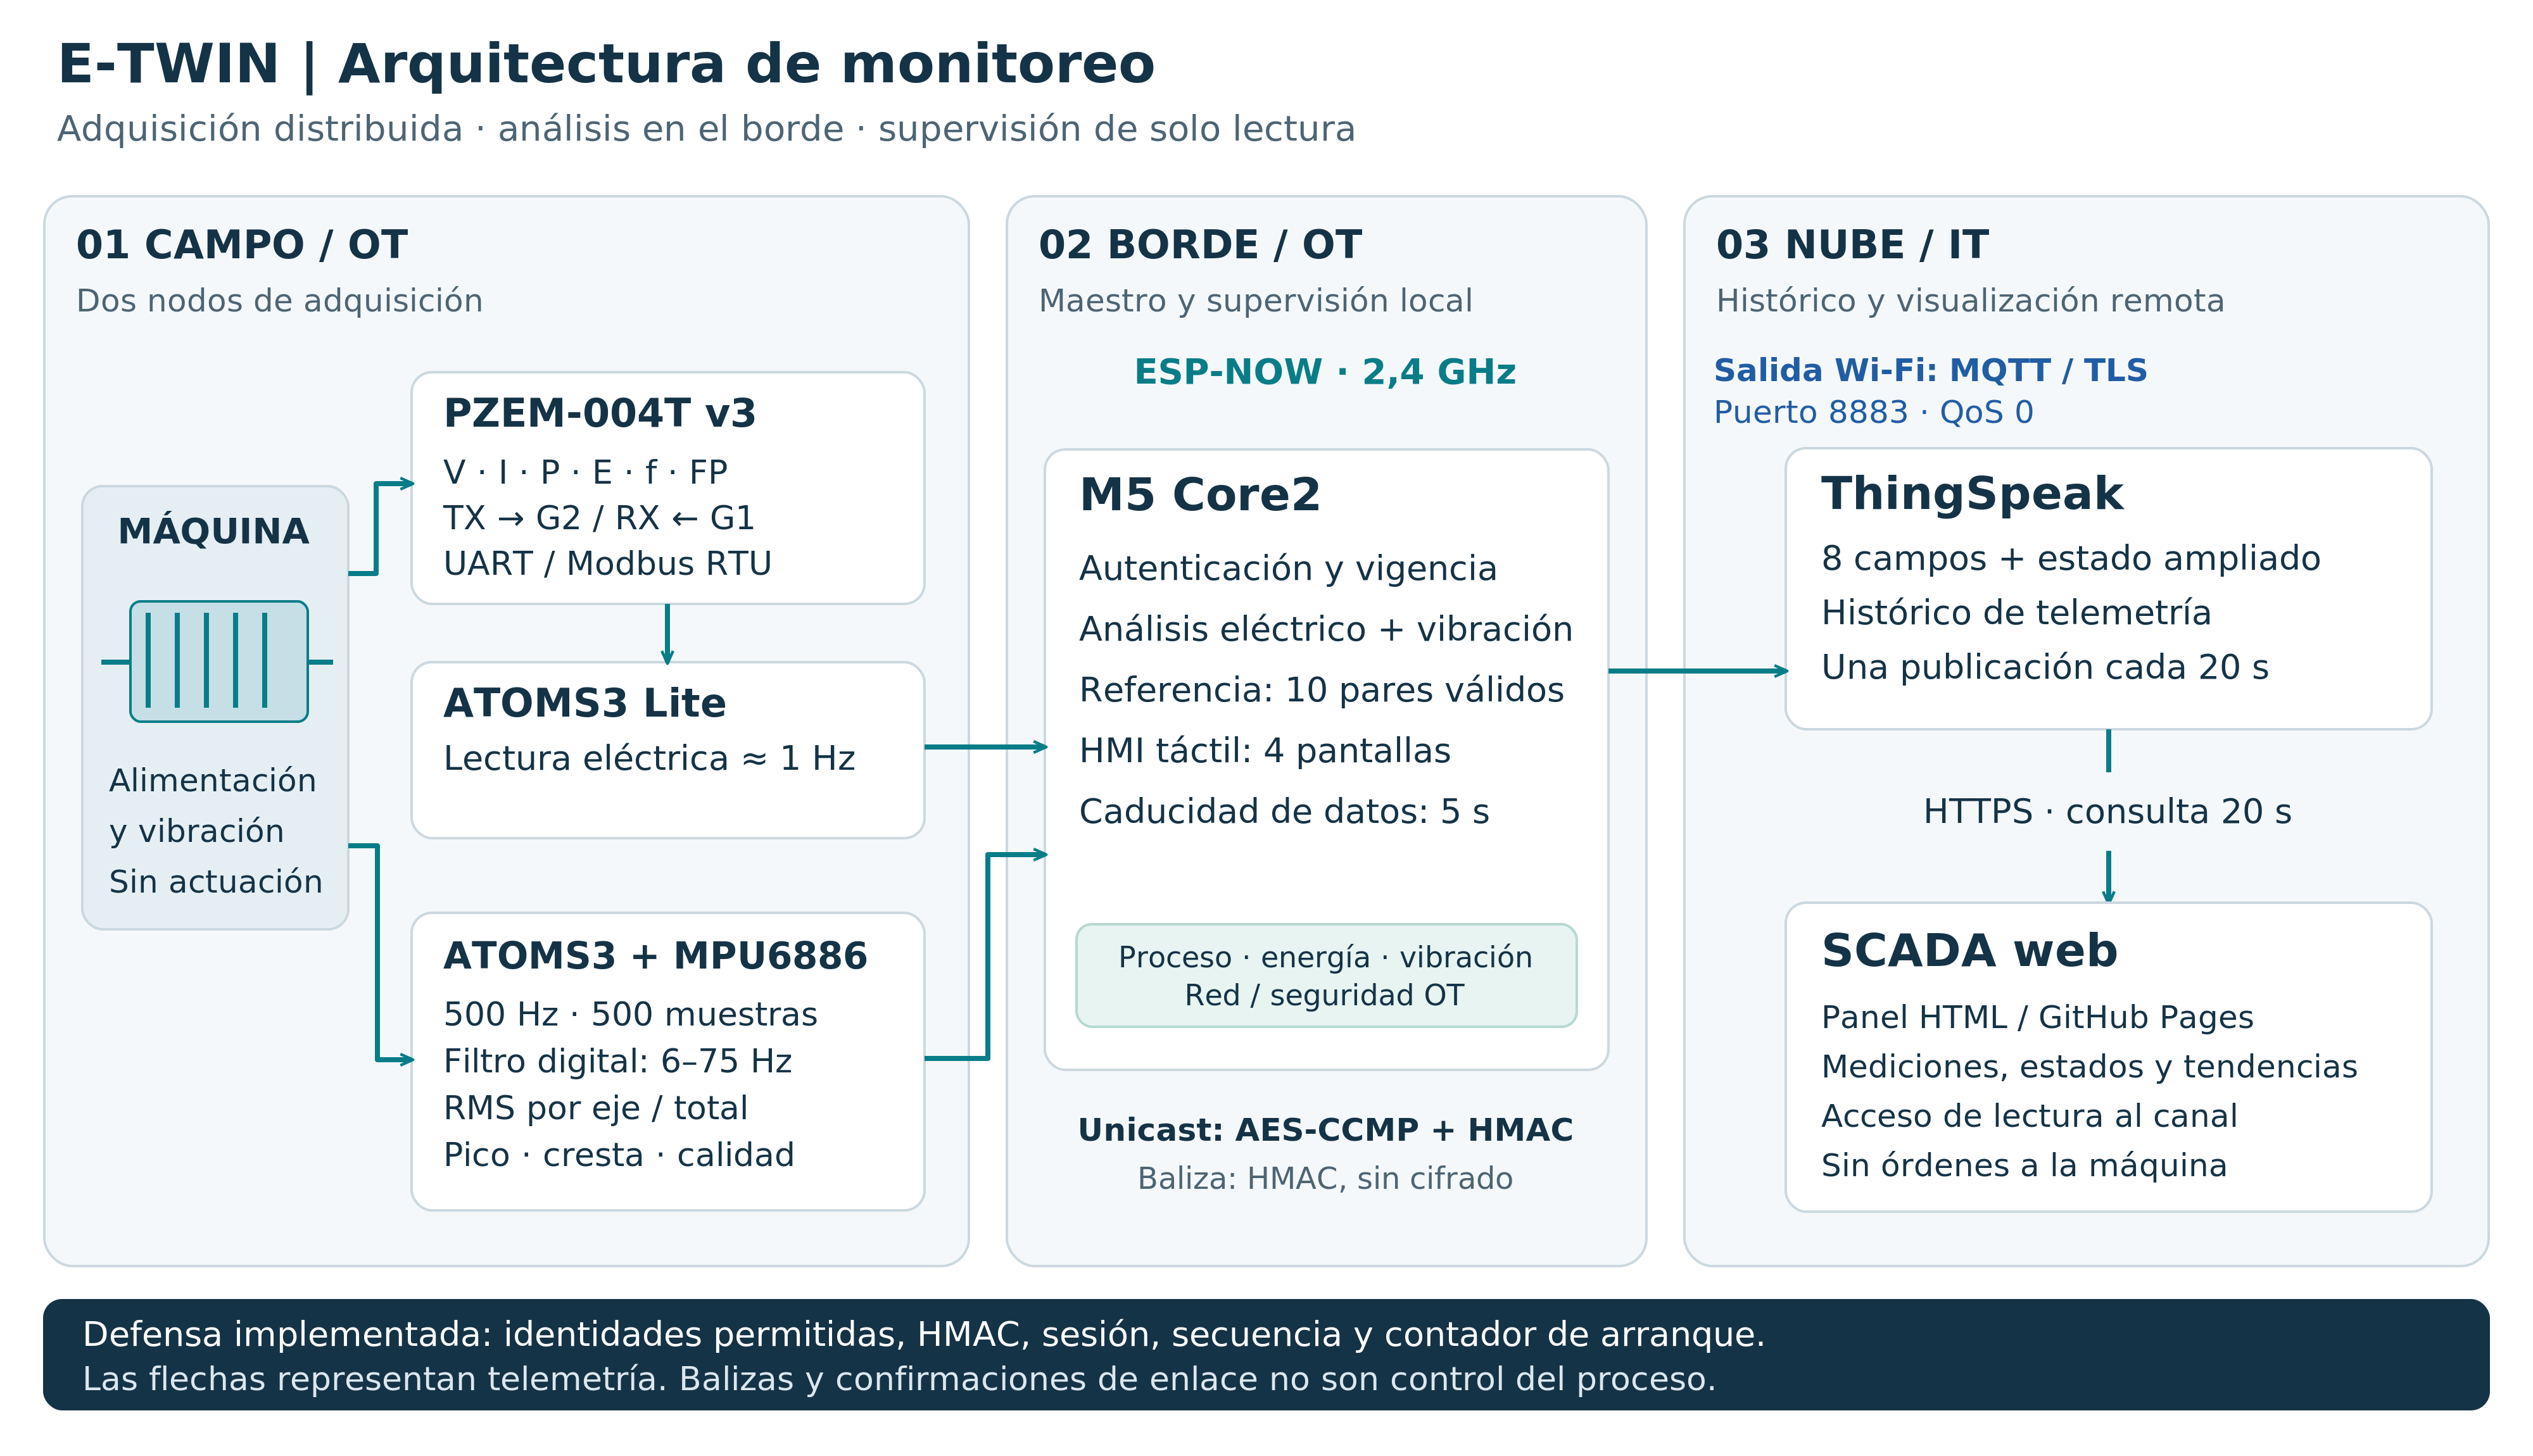
\includegraphics[width=\linewidth]{arquitectura_etwin.png}
\caption{Arquitectura implementada de E-TWIN. Las zonas representan funciones, no una segmentación de red ya demostrada. La aplicación web no dispone de una ruta de actuación sobre la máquina.}
\label{fig:architecture}
\end{figure}

ESP-NOW permite el intercambio local sin que los nodos necesiten conectarse a la nube. Se emplean pares unicast cifrados y una baliza autenticada para localizar el canal del maestro. El canal de esta red comparte la radio con la conexión Wi-Fi de la pasarela, restricción que condiciona la configuración y la recuperación del enlace~\cite{espnow}. Las tramas de energía y vibración ocupan 68 y 76 bytes, respectivamente, incluida su etiqueta de autenticación; no se transmite la señal inercial cruda.

El M5 Core2 integra los datos y una interfaz con cuatro vistas: proceso, energía, vibración y comunicaciones/OT. La navegación se realiza mediante gestos horizontales y controles táctiles. El esquema animado expresa estados de operación, no una velocidad de giro medida. Una tarea de comunicación publica cada 20 s en ThingSpeak mediante MQTT/TLS, puerto 8883. La plataforma utiliza QoS 0~\cite{thingspeak}; por ello, el envío no equivale a una confirmación de almacenamiento. La aplicación HTML consulta por HTTPS, ofrece tendencias y exportación, y marca como antigua la información que supera 65 s.

\subsection{Procesamiento de vibración}
La IMU se configura a $\pm8g$, con filtro interno de 99 Hz y muestreo nominal de 500 Hz. La lectura mediante FIFO se desacopla del refresco de pantalla y de la radio. El firmware contempla 1500 muestras de estabilización, aproximadamente 3 s. Se invalidan ventanas con saturación, error del sensor, desbordamiento o temporización fuera de tolerancia.

El filtrado se aplica a cada eje con signo antes de calcular la norma. Consiste en un pasaaltos Butterworth de cuarto orden a 6 Hz y un pasabajos de cuarto orden a 75 Hz: cuatro secciones biquad por eje, de octavo orden total en cascada. El primero reduce la componente estática y las variaciones lentas; el segundo limita el contenido de alta frecuencia. No se resta un nivel de ruido arbitrario ni se recortan impactos para producir una curva artificialmente estable. Para $N=500$ muestras filtradas $\widetilde{a}_{j,k}$, se calcula
\begin{align}
 a_{j,\mathrm{RMS}}&=\sqrt{\frac{1}{N}\sum_{k=1}^{N}\widetilde{a}_{j,k}^{\,2}},\quad j\in\{x,y,z\},\\
 a_{\mathrm{RMS}}&=\sqrt{a_{x,\mathrm{RMS}}^2+a_{y,\mathrm{RMS}}^2+a_{z,\mathrm{RMS}}^2},\\
 a_{\mathrm{pico}}&=\max_k\sqrt{\widetilde{a}_{x,k}^2+\widetilde{a}_{y,k}^2+\widetilde{a}_{z,k}^2},\qquad
 C_f=\frac{a_{\mathrm{pico}}}{a_{\mathrm{RMS}}}.
\end{align}
La aceleración se expresa en m/s\textsuperscript{2}; no se interpreta como velocidad RMS en mm/s ni se usa para clasificar severidad según normas de vibración. El ancho de banda restringe el alcance a fenómenos presentes en esa banda. Sin señales crudas antes y después del filtro no puede cuantificarse la mejora real de relación señal/ruido del ensayo.

\subsection{Análisis operativo y referencia de diez pares}
La Fig.~\ref{fig:flow} resume el tratamiento de calidad. El maestro estima potencia aparente $S=VI$, desviación relativa de potencia $\Delta P=100(P/P_0-1)$ y relación de vibración $R_a=a_{\mathrm{RMS}}/a_0$. Los valores $P_0$ y $a_0$ provienen de diez pares nuevos y válidos, separados al menos un segundo, adquiridos tras una orden local. La captura se cancela ante pérdida de datos o reinicios y se rechaza si la variación excede los coeficientes configurados: 0,15 para potencia y 0,30 para vibración. Una referencia aceptada se conserva en memoria no volátil.

\begin{figure}[!htbp]
\centering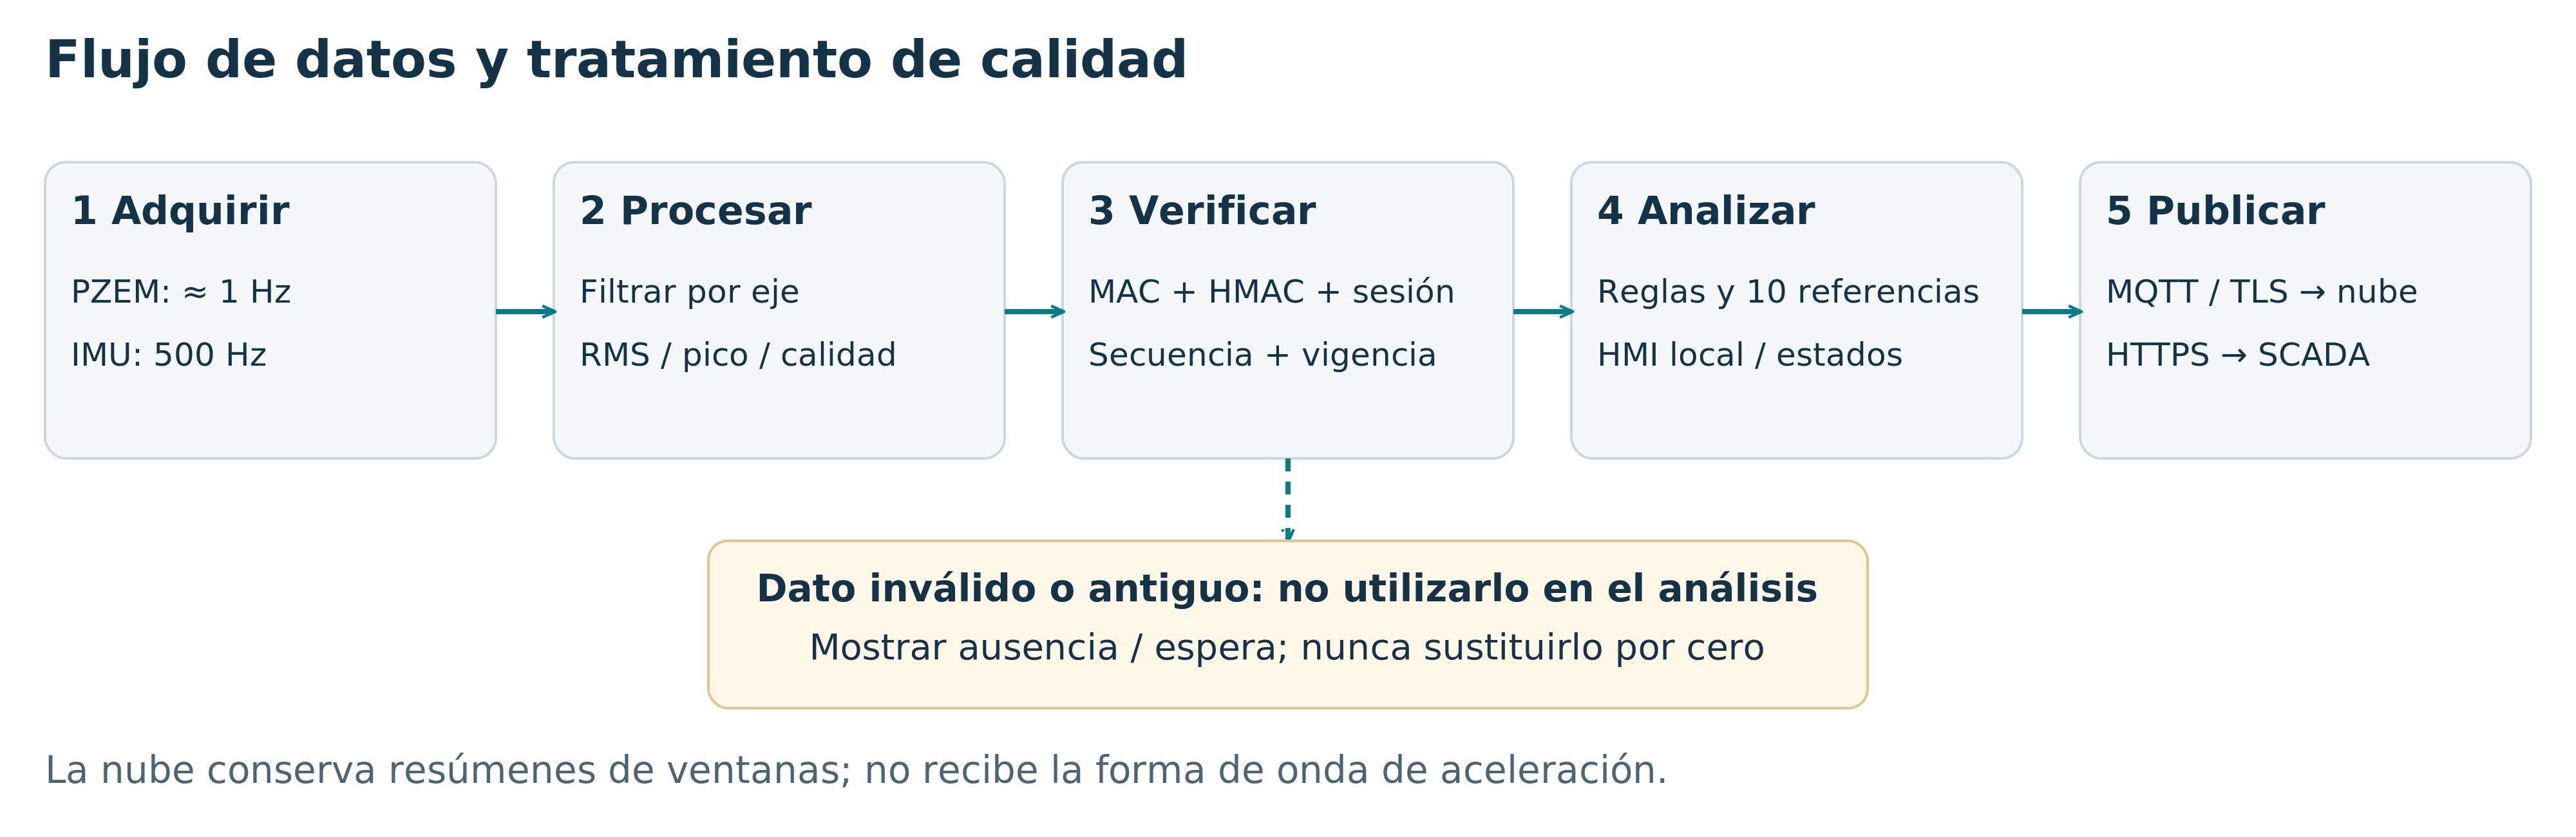
\includegraphics[width=\linewidth]{flujo_datos.png}
\caption{Flujo funcional y control de calidad. La ausencia de una lectura no se presenta como consumo o vibración nulos.}
\label{fig:flow}
\end{figure}

La referencia aprendida es una condición de comparación, no una calibración del sensor. Se exige carga, velocidad y montaje comparables para interpretar sus diferencias. Los umbrales iniciales son 20\% de incremento de potencia y relaciones de vibración de 1,5 y 2 para advertencia y alarma. El factor de potencia se supervisa por debajo de 0,80 cuando la potencia supera 50 W. En la configuración suministrada, la tensión nominal y la alarma absoluta de vibración permanecen desactivadas. Estas reglas requieren adaptación a la máquina; no constituyen un diagnóstico de averías. Tampoco se calcula eficiencia mecánica, pues faltan potencia útil, torque y velocidad.

\subsection{Ciberseguridad OT y privacidad}
El diseño considera falsificación de telemetría, modificación de paquetes, repetición de mensajes, exposición de credenciales y uso de datos antiguos. La defensa combina lista de MAC permitidas, validación de tipo y longitud, cifrado AES-CCMP de unicast, HMAC-SHA256 truncado a 128 bits, identificador de sesión, secuencia y contador de arranque persistente. Las balizas de descubrimiento no están cifradas: su autenticidad se verifica con HMAC. Esta distinción es relevante porque ESP-NOW no cifra difusión/multidifusión~\cite{espnow}.

El enlace con la nube valida un certificado de autoridad y requiere una hora válida para TLS. El canal permite separar las credenciales de publicación de la lectura del panel. El firmware no incorpora órdenes de control desde la nube; las entradas inválidas caducan sin modificar actuadores. El repositorio público excluye las credenciales de Wi-Fi/MQTT y las claves de radio, e incluye un generador local. Los datos estudiados no contienen coordenadas, aunque un histórico de consumo puede revelar horarios de actividad; su publicación requiere una decisión del responsable de la instalación.

Estos controles reducen superficie de exposición, pero no demuestran conformidad con NIST ni una arquitectura Zero Trust completa. No se verificaron ataques de radio, extracción de claves, arranque seguro, cifrado de flash, actualizaciones firmadas ni segmentación mediante VLAN. Además, las claves están disponibles al firmware y no aisladas por hardware; una intrusión física tiene consecuencias distintas de una alteración de paquete. La separación OT/IT y el acceso restringido a los equipos deben completarse para un despliegue productivo~\cite{nist2023}.

\FloatBarrier
\section{Resultados}
\subsection{Evidencia funcional del prototipo}
La Fig.~\ref{fig:physical} documenta los componentes y las vistas locales; las Figs.~\ref{fig:web} y~\ref{fig:quality} muestran la interfaz web del equipo. Se distinguen los indicadores eléctricos, la animación del proceso, los datos inerciales por eje y los estados de comunicación. Las imágenes se incorporan como evidencia original, con recortes de encuadre sin alterar cifras. No se utiliza la animación como evidencia de una magnitud física no medida.

\begin{figure}[!htbp]
\centering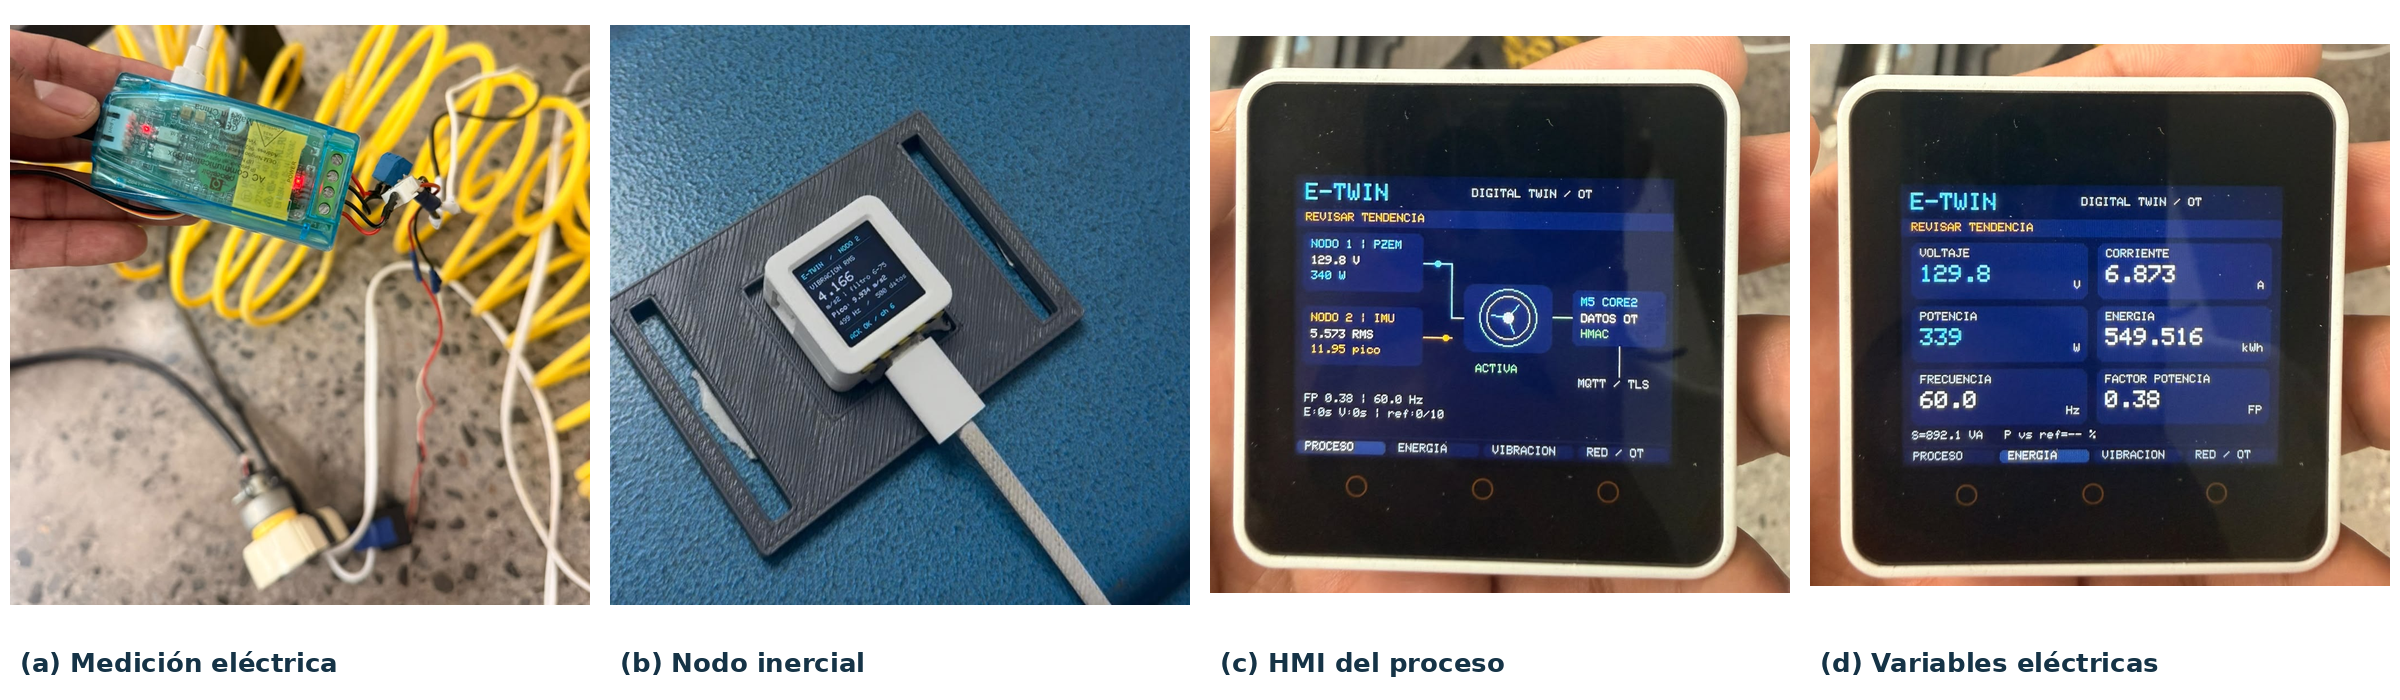
\includegraphics[width=\linewidth]{prototipo_fisico.png}
\caption{Fotografías del prototipo suministradas por el equipo: (a) módulo de medición eléctrica, (b) ATOMS3 sobre soporte, (c) supervisión del proceso y (d) lecturas eléctricas en el M5 Core2. No se presume sincronización con la ventana estadística.}
\label{fig:physical}
\end{figure}

\begin{figure}[!htbp]
\centering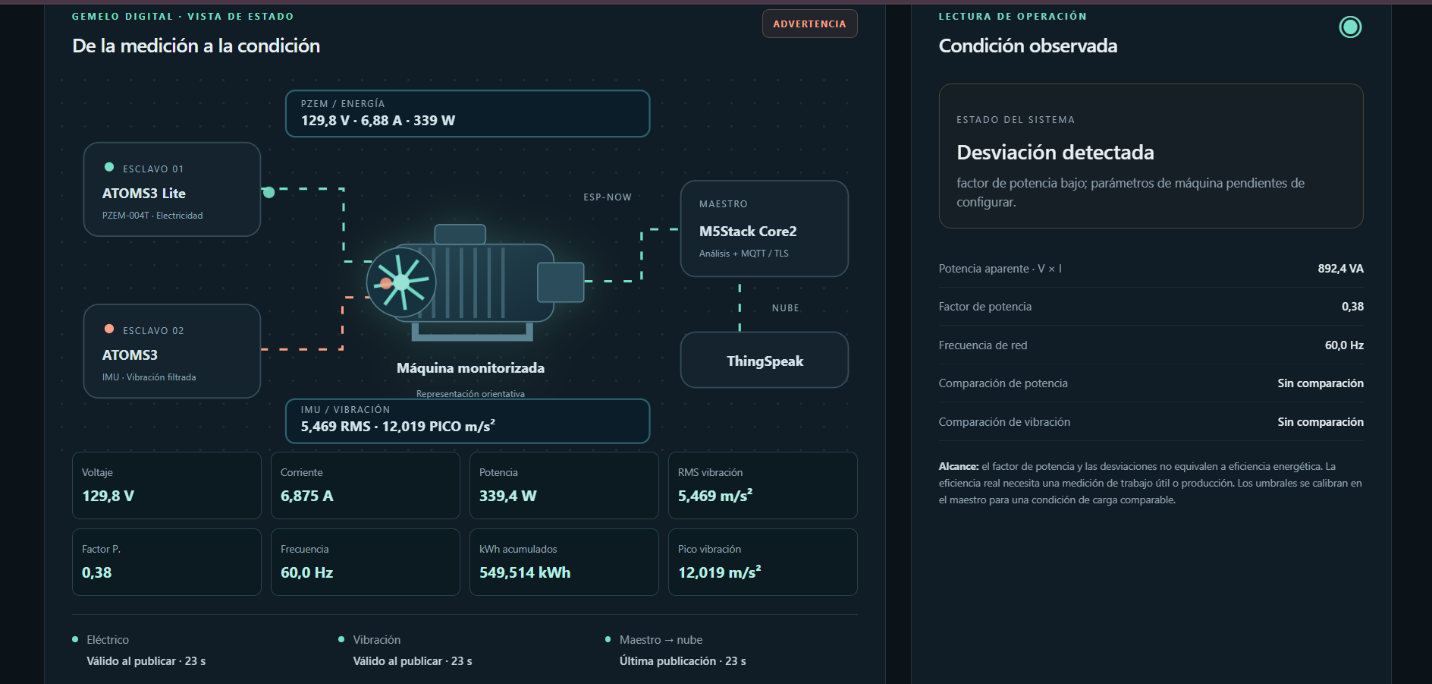
\includegraphics[width=0.96\linewidth]{scada_proceso.png}
\caption{Captura original del SCADA web: relación entre nodos, activo representado, variables eléctricas y vibración. Las cifras corresponden a la captura, no necesariamente a las medias de la Tabla~\ref{tab:stats}.}
\label{fig:web}
\end{figure}

\begin{figure}[!htbp]
\centering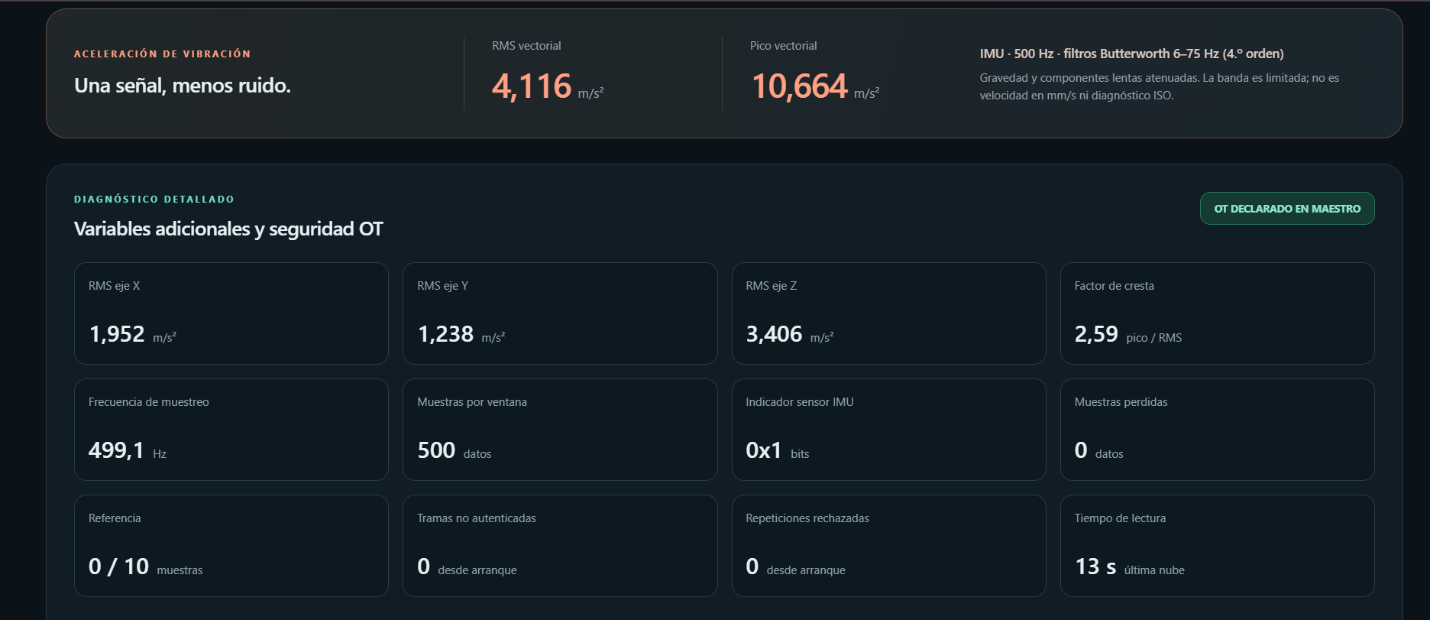
\includegraphics[width=0.96\linewidth]{scada_calidad.png}
\caption{Captura original de variables ampliadas y calidad. El contador de referencia 0/10 corresponde al instante de esta imagen; el CSV permite observar posteriormente una referencia aceptada.}
\label{fig:quality}
\end{figure}

\subsection{Comportamiento en la ventana seleccionada}
La Tabla~\ref{tab:stats} resume las 31 observaciones. La tensión permaneció entre 129,6 y 129,9 V y la corriente entre 6,770 y 6,867 A. La potencia media fue 341,15 W, con un máximo de 373,0 W que se conserva en la Fig.~\ref{fig:power}. La potencia aparente media calculada fue 883,72 VA. El factor de potencia bajo describe la relación entre potencia activa y aparente; no permite concluir que la eficiencia del motor sea del 38\%.

\begin{table}[!htbp]
\centering\caption{Estadística descriptiva de los últimos diez minutos conjuntos válidos ($n=31$). $s$ es desviación estándar muestral, no incertidumbre de medición.}
\label{tab:stats}
\small\setlength{\tabcolsep}{8pt}
% Generado automáticamente por analysis/analyze_csv.py; s = desviación muestral.
\begin{tabular}{llrrrr}\toprule
Variable & Unidad & Media & $s$ & Mínimo & Máximo\\\midrule
Tensión & V & 129,79 & 0,09 & 129,60 & 129,90 \\
Corriente & A & 6,809 & 0,029 & 6,770 & 6,867 \\
Potencia activa & W & 341,15 & 8,02 & 337,30 & 373,00 \\
Energía acumulada & kWh & 549,548 & 0,017 & 549,520 & 549,577 \\
Frecuencia & Hz & 59,974 & 0,044 & 59,900 & 60,000 \\
Factor de potencia & -- & 0,384 & 0,010 & 0,380 & 0,420 \\
Aceleración RMS & m/s$^2$ & 4,736 & 0,928 & 3,201 & 6,596 \\
Aceleración pico & m/s$^2$ & 10,283 & 1,891 & 6,835 & 13,871 \\
\bottomrule\end{tabular}

\end{table}

\begin{figure}[!htbp]
\centering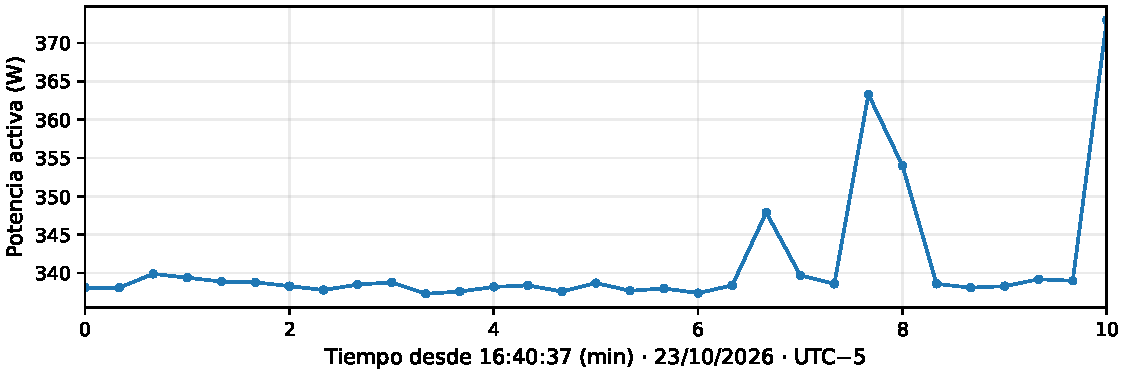
\includegraphics[width=0.94\linewidth]{potencia_10min.pdf}
\caption{Potencia activa sin suavizado adicional ni eliminación de extremos. Cada punto corresponde a una publicación válida del CSV.}
\label{fig:power}
\end{figure}

La aceleración RMS media fue 4,736 m/s\textsuperscript{2}, frente a un pico medio de 10,283 m/s\textsuperscript{2} (Fig.~\ref{fig:vibration}). Sus coeficientes de variación fueron 19,59\% para RMS y 2,35\% para potencia. Esa diferencia describe variabilidad observada; no identifica una falla ni prueba causalidad entre ambas señales. La tasa inercial estimada se situó entre 498,0 y 499,1 Hz, con 500 muestras por ventana y cero pérdidas declaradas en todas las publicaciones válidas.

\begin{figure}[!htbp]
\centering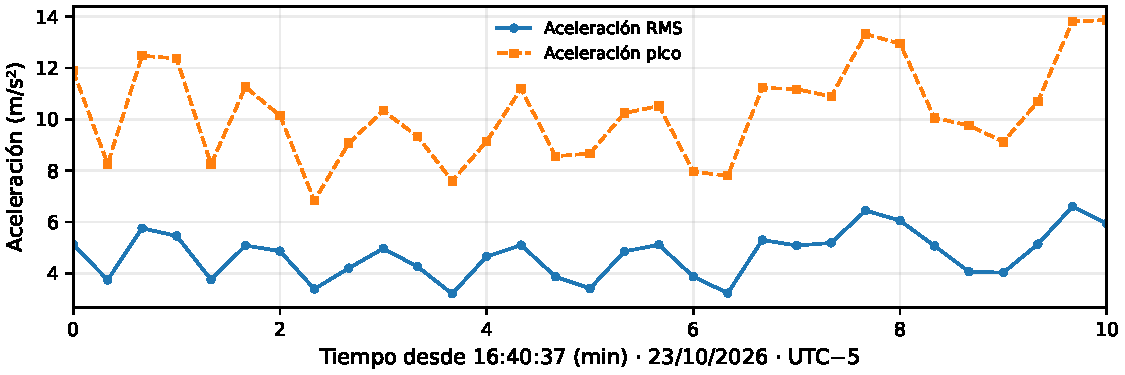
\includegraphics[width=0.94\linewidth]{vibracion_10min.pdf}
\caption{Indicadores de aceleración resultante de ventanas filtradas de 500 muestras. El muestreo de esta gráfica es de 20 s y no representa la forma de onda de 500 Hz.}
\label{fig:vibration}
\end{figure}

Los 30 intervalos de publicación fueron exactamente de 20 s. Las edades de los nodos al publicar fueron 163--799 ms para energía y 46--977 ms para vibración, inferiores al umbral de vigencia. La ausencia de huecos describe completitud de la ventana seleccionada; no equivale a una tasa de entrega de ESP-NOW del 100\% ni a disponibilidad global del sistema.

Todas las filas conservaron \texttt{WARN} y máscara 34: advertencia por factor de potencia y configuración pendiente. La primera publicación con \texttt{ref=1} y \texttt{ct=10} aparece a las 16:46:37; hay 13 registros posteriores con referencia disponible. No se reconstruyen las diez observaciones locales de captura a partir de diez publicaciones de nube. Tras la referencia, la desviación publicada de potencia abarcó $-0,2$ a 10,4\% y la razón de vibración 0,73--1,50. Este último valor está redondeado; no se activó un bit de alarma de vibración en la serie.

\subsection{Consistencia interna de las lecturas}
Como control eléctrico se evaluó
\begin{equation}
 d_{P,i}=100\,\frac{|P_i-V_iI_i\mathrm{FP}_i|}{P_i},
\end{equation}
con $P_i>0$. La discrepancia media fue 0,721\% y la máxima 1,233\%. Este control identifica incompatibilidades entre campos, pero todas sus entradas proceden del mismo PZEM y el factor de potencia está redondeado. Por tanto, no estima error frente al valor verdadero.

El contador pasó de 549,520 a 549,577 kWh, de modo que el incremento del ensayo fue $\Delta E=0,057$ kWh, no 549,577 kWh. La energía calculada desde potencia se obtuvo mediante
\begin{equation}
 E_P=\frac{1}{3{,}6\times10^6}\sum_{i=1}^{n-1}\frac{P_i+P_{i+1}}{2}(t_{i+1}-t_i),
\end{equation}
con potencia en W, tiempo en s y resultado en kWh. Se obtuvo $E_P=0,0567781$ kWh. La diferencia fue 0,22194 Wh, equivalente a 0,389\% del incremento del contador (Fig.~\ref{fig:energy}). El contador se exporta con resolución de 0,001 kWh y la potencia está submuestreada cada 20 s; la coincidencia no constituye una mejora de exactitud frente a otro instrumento.

\begin{figure}[!htbp]
\centering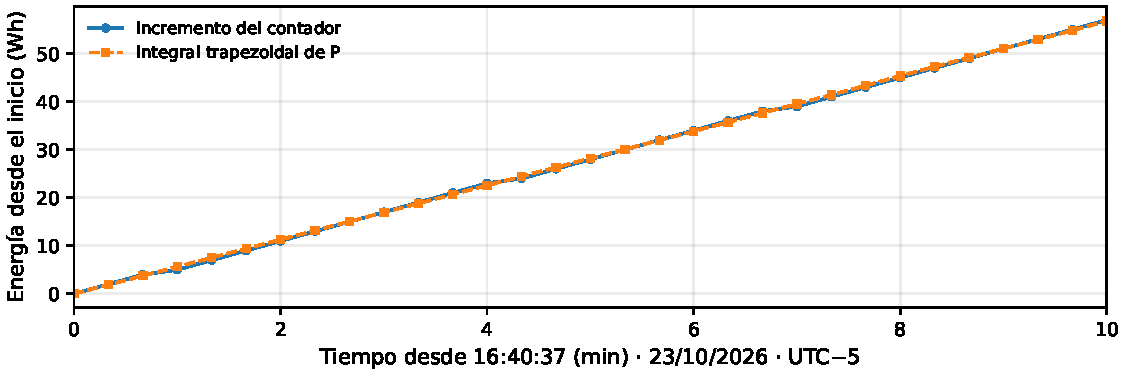
\includegraphics[width=0.94\linewidth]{energia_10min.pdf}
\caption{Incremento del contador frente a integración de potencia sobre los mismos instantes. Se compara energía relativa al inicio; ambas series proceden de la misma cadena de medición.}
\label{fig:energy}
\end{figure}

La identidad $a_{\mathrm{RMS}}=\sqrt{a_x^2+a_y^2+a_z^2}$ presentó una diferencia máxima de 0,000607 m/s\textsuperscript{2}; la relación pico/RMS difirió del factor de cresta publicado en menos de 0,00486. Ambas diferencias son compatibles con la precisión decimal exportada. No contrastan el acelerómetro con un excitador o patrón independiente.

\subsection{Contraste con el antecedente y pruebas de software}
El estudio de Varela-Aldás \textit{et al.}~\cite{varela2022} compara dos canales PZEM con un Emporia Gen 2 Vue durante siete días. Sus tablas reportan errores relativos medios de potencia de 2,1059\% y 1,9487\%, y de energía de 0,8137\% y 1,3627\%. Estos valores pertenecen a aquel montaje. En E-TWIN se dispone de diez minutos sin referencia independiente: el 0,389\% calculado es discrepancia interna entre contador e integral, no un error homologable. El antecedente aporta el criterio de evaluación comparativa, no un factor de corrección aplicable al CSV. La Tabla~\ref{tab:evidence} delimita qué evidencia respalda cada conclusión.

\begin{table}[!htbp]
\centering\caption{Alcance de la verificación realizada en E-TWIN.}
\label{tab:evidence}\small
\begin{tabularx}{\linewidth}{p{0.21\linewidth}XX}\toprule
Evidencia & Resultado & Alcance permitido\\\midrule
Núcleo del software & 145 comprobaciones; cero fallos. & Contratos, autenticación, estados y lógica cubiertos por las pruebas de anfitrión.\\
Filtro digital & Pruebas sintéticas de continua, respuesta frecuencial, RMS, ventanas y reinicio aprobadas. & Corrección numérica; no calibración física de la IMU.\\
Panel web & Pruebas de datos y de interfaz simulada aprobadas. & Tratamiento de ausencias, estados y flujo de interfaz; no ensayo integral de navegadores.\\
CSV y evidencias & 31 registros conjuntos y fotografías/capturas originales. & Funcionamiento documentado durante el intervalo observado.\\
Metrología y seguridad de campo & Sin patrón simultáneo ni campaña adversarial. & Exactitud, inmunidad a ataques y desempeño prolongado pendientes.\\\bottomrule
\end{tabularx}
\end{table}

Las pruebas del filtro, ejecutadas con una sinusoide de amplitud unitaria, produjeron RMS de 0,707079 a 20 Hz y aproximadamente 0,500000 a 75 Hz; esta caída es coherente con la frecuencia de corte. El residuo ante componente continua fue aproximadamente $1,4\times10^{-6}$ m/s\textsuperscript{2} en el ensayo sintético. La atenuación fuera de banda demuestra la operación del algoritmo, pero también confirma que no deben compararse RMS obtenidos con bandas distintas. La compilación y carga del firmware no se repitieron en esta evaluación documental; el registro de pruebas incluido corresponde a ejecución en anfitrión.

Tras la ventana, la publicación de las 16:50:57 conserva vibración válida pero no energía; las tres siguientes invalidan ambos nodos y muestran \texttt{WAIT}. Esta evidencia ilustra que la aplicación no rellena ausencias con cero. No permite atribuir la causa a desconexión física, fallo del sensor o pérdida de radio, ni medir recuperación ante una interrupción controlada. Los contadores \texttt{rj} y \texttt{rp} permanecen en cero dentro de la ventana: no prueban resistencia frente a intentos de intrusión.

\FloatBarrier
\section{Discusión: impacto, viabilidad y escalabilidad}
El beneficio previsto es ofrecer una primera capa de observación combinada para equipos que no disponen de telemetría integrada. La visualización local favorece inspecciones junto a la máquina y el histórico facilita revisar variaciones después del evento. El uso productivo debe concentrarse inicialmente en tendencias y comparación de condiciones semejantes. No se han medido ahorro económico, reducción de paradas ni mejora de productividad; tales resultados requieren una línea base operativa y seguimiento longitudinal.

La viabilidad técnica se apoya en una adquisición modular y procesamiento en el borde: el sensor inercial resume 500 muestras antes de transmitir y la pasarela mantiene separadas las tareas de interfaz y nube. El sistema no depende de enviar señales crudas para visualizar RMS y picos. Sin embargo, la pasarela es un punto único de fallo, y el uso compartido del canal Wi-Fi condiciona el enlace local. La operación local sin Internet está contemplada en el diseño, pero debe validarse con ensayos controlados. No existe una cola histórica para recuperar todos los intervalos perdidos durante una caída de la nube.

La viabilidad económica debe estimarse mediante una lista verificable de materiales: tres dispositivos, PZEM y transformador de corriente según versión, fuentes, cableado, soportes y envolventes. No se asigna un costo total porque no se aportaron facturas ni cotizaciones. La instalación requiere competencias en medición eléctrica, montaje mecánico y redes; el mantenimiento incluye verificar fijaciones, actualizar certificados y gestionar credenciales. La publicación del panel y del código no debe exponer contraseñas ni registros sensibles de producción.

La replicabilidad exige registrar la placa de la máquina, ubicación y orientación del acelerómetro, condiciones de carga y método de fijación. La banda 6--75 Hz es una decisión del prototipo, no un ajuste universal. Una máquina con fenómenos relevantes fuera de ella requiere otra adquisición y una nueva referencia. Las fotografías no identifican de manera suficiente el modelo o la potencia nominal del equipo, por lo que no se generalizan los valores observados a una clase de motores.

La escalabilidad no consiste únicamente en añadir pares de radio. Deben dimensionarse el número de dispositivos, ocupación del canal, tamaño de mensajes, almacenamiento y reglas de caducidad. Una arquitectura ampliada requeriría identidades y claves provisionadas por dispositivo, segmentación de red y un backend apropiado para múltiples activos. Los ocho campos de ThingSpeak se reservan a las mediciones principales; el estado ampliado debe versionarse y respetar su límite de tamaño. La visualización pública es adecuada para demostración con datos autorizados, no necesariamente para un entorno industrial con horarios y consumos confidenciales.

La principal limitación experimental es la brevedad del intervalo y la ausencia de señales crudas, patrón simultáneo y etiquetas de estados mecánicos. Con 31 publicaciones no es posible construir ni evaluar un clasificador de fallas, demostrar mantenimiento predictivo o caracterizar latencia de red. A cambio, la selección explícita, la preservación de extremos y la separación entre consistencia y exactitud permiten auditar los resultados sin ocultar esas restricciones.

\section{Conclusiones y trabajo futuro}
E-TWIN integra dos nodos ESP-NOW con una pasarela M5 Core2, supervisión táctil y acceso web de solo lectura. La propuesta relaciona parámetros eléctricos e indicadores inerciales mediante un contrato que exige calidad y vigencia, añade una referencia operativa de diez pares y aplica autenticación, cifrado unicast y controles contra repetición. Su representación digital refleja el estado observado; no reemplaza un modelo físico validado ni un sistema de protección.

En la ventana cerrada de diez minutos se conservaron 31 publicaciones completas, con potencia media de 341,15 W, aceleración RMS media de 4,736 m/s\textsuperscript{2} e incremento energético de 57 Wh. La integración de potencia produjo 56,7781 Wh y una discrepancia interna de 0,389\%. Los resultados acreditan coherencia de la cadena de datos y comportamiento funcional documentado, sin establecer exactitud metrológica o condición mecánica saludable. Las pruebas de anfitrión aportan evidencia adicional sobre la lógica del software, no sobre todos los escenarios de campo.

La siguiente validación debe registrar simultáneamente el prototipo y un instrumento eléctrico independiente, bajo varias cargas, durante un período prolongado; se reportarán sesgo, error absoluto y relativo, sincronización e incertidumbre de la referencia. Para vibración se requiere un montaje reproducible, adquisición cruda y contraste con acelerometría de referencia. Se propone además documentar pruebas de pérdida de red, recuperación, mensajes alterados y repetidos, y completar provisión de claves, arranque seguro y actualización firmada. Solo después de identificar la máquina y reunir estados etiquetados será justificable evaluar modelos predictivos y beneficios operativos.

\section*{Disponibilidad del material}
El paquete reproducible incluye el firmware suministrado sin secretos, el panel web, los datos originales y seleccionados, los scripts de análisis, las figuras y las fuentes LaTeX. El archivo \texttt{README.md} incorpora una imagen enlazada a la demostración indicada por el equipo: \href{https://youtu.be/txEMzoSkKmY}{video de E-TWIN}. Las identidades de autores, afiliación, correos y tutor se completan en \texttt{metadatos.tex}; no se deducen de la autoría del antecedente bibliográfico.

\bibliographystyle{IEEEtran}
\bibliography{referencias}
\end{document}
